% -- Encoding UTF-8 without BOM
% -- XeLaTeX => PDF (BIBER)

\documentclass[print]{cv-style}

\sethyphenation[variant=british]{english}{}

\usepackage{fontspec}
\usepackage{fontawesome}
\usepackage{enumitem}
\setlist{leftmargin=5.5mm}

\begin{document}

\header{}{Paul Chote}{Curriculum Vitae}

\begin{aside}
\vspace{0.35cm}~
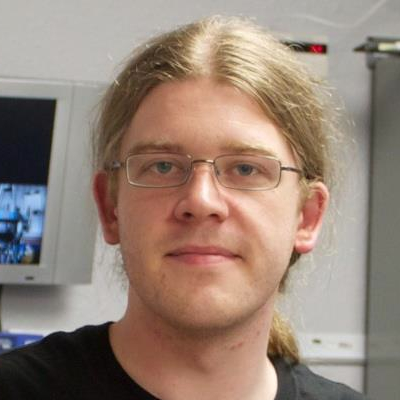
\includegraphics[width=3.6cm]{CV_Photo.jpg}
~
\section{Contact}
Department of Physics
University of Warwick
Gibbet Hill Road
Coventry
CV4 7AL
UK
~
{\bf mobile:} 
+44 7481 178055
{\bf work:} 
+44 2476 151862
{\bf email:}
{\small p.chote@warwick.ac.uk}
{\small paul@chote.net}
{\bf skype:}
{\small pchote}
~
\section{Links}
{\small \faLinkedin~linkedin.com/in/pchote}
{\small \faGithub~github.com/pchote}
~
\section{Computing}
\vspace{1mm}{\bf Operating systems:} 
{\small Linux, macOS, Windows}
\vspace{1mm}{\bf Programming Languages:} 
{\small C, C\#, Python, Bash,\\HTML, CSS, Javascript,\\Objective-C, Lua}
\vspace{1mm}{\bf Display APIs:} 
{\small OpenGL, PGPLOT, Matplotlib}
\vspace{1mm}{\bf Embedded Systems:}
{\small AVR, ARM}
\vspace{1mm}{\bf Web Frameworks:}
{\small Flask, Django, JQuery}
\vspace{1mm}{\bf Grid Computing:} 
{\small SGE, Condor, DRMAA}
\vspace{1mm}{\bf Version Control:} 
{\small Git, SVN}
\vspace{1mm}{\bf Word Processing:} 
{\small \LaTeX, Microsoft Office}
~
\end{aside}

%----------------------------------------------------------------------------------------
\vspace{0.5cm}
\section{Education}
\vspace{-7mm}
\begin{entrylist}
\vspace{2mm}
\entry{}{}{Victoria University of Wellington (VUW), New Zealand}{\vspace{-0.5cm}}
\entry{2011~--~2014}{Doctor of Philosophy {\normalfont in Physics}}{}{\vspace{-0.5cm}}
\entry{2009~--~2010}{Master of Science {\normalfont in Physics with Distinction}}{}{\vspace{-0.5cm}}
\entry{2008~--~2009}{Bachelor of Science {\normalfont in Physics with First Class Honours}}{}{\vspace{-0.5cm}}
\entry{2005~--~2007}{Bachelor of Science {\normalfont in Mathematics and Physics}}{}{\vspace{-0.5cm}}
\end{entrylist}

%----------------------------------------------------------------------------------------

\section{Experience}

\begin{entrylist}
%------------------------------------------------
\entry
  {2015--2018}{Department of Physics, Warwick University}{Coventry, United Kingdom}
  {\jobtitle{Postdoctoral Research Fellow}\\
  \vspace{-3mm}
  \it{Repair and automation of a 1m research telescope:}\vspace{-1mm}\\
  \begin{itemize}
    \item Identified optical and mechanical faults and developed repair strategies.
    \item Developed hardware and low-level software interfaces for observatory systems.
    \item Designed and implemented data management and calibration pipeline.
    \item Developed web dashboards and tools using Python, Flask, and Django.
  \end{itemize}
  \it{Identification of targets of interest in wide-area astronomical surveys:}
  \begin{itemize}
    \item Developed a data analysis pipeline to clean observations from the \it{iPTF} survey and quantify photometric variability of stars from input catalogs.
    \item Developed a real-time analysis pipeline to detect transient astrophysical events and variable stars in the \it{NGTS} survey.
  \end{itemize}
  Acquired and analysed data of variable white dwarf stars.
}
%------------------------------------------------
\entry
  {2014--2015}{School of Chemical and Physical Sciences, VUW}{Wellington, New Zealand}
  {\jobtitle{Research Assistant: 2D X-Ray Dosimeter Development}
  \begin{itemize}
    \item Developed a 2D readout instrument for X-Ray sensitive films, adapting a 3D printer to hold a scanning laser and photon counting electronics.
    \item Characterised system properties including resolution, linearity, and noise levels.
    \item Created and characterised X-ray sensitive films in the lab.
  \end{itemize}
}
%------------------------------------------------
\entry{2011~--~2014}{School of Chemical and Physical Sciences, VUW}{Wellington, New Zealand}
  {\jobtitle{PhD. Research: CCD Time-Series Photometry of White Dwarf Stars}
\begin{itemize}
    \item Developed high-speed CCD time-series photometer instruments used with a 1\,m telescope at Mt John observatory in New Zealand and the 2.1\,m telescope at McDonald observatory in the USA.
    \item Created a CCD data reduction pipeline for real-time analysis and visualisation.
    \item Acquired time-series photometry of variable white dwarf (WD) targets.
    \item Analysis of targets included identification of WD pulsation modes, investigation of pulsation stability, and the consideration of convection effects.
\end{itemize}}
%------------------------------------------------
\entry{2009~--~2010}{School of Chemical and Physical Sciences, VUW}{Wellington, New Zealand}
  {\jobtitle{MSc. Research: A Semi-Analytical Model for Gravitational Microlensing}
\begin{itemize}
    \item Investigated techniques for calculating gravitational microlensing light curves.
    \item Developed and implemented a computationally efficient semi-analytical model for simulating gravitational microlensing events with up to four lens bodies.
    \item Implemented model support for orbital motion effects in the source, lens, and observer systems.
  \end{itemize}}
%------------------------------------------------
\entry{\small Summer 2008}{\small Research School of Astronomy and Astrophysics, Australian National University}{Canberra, Australia}
  {\jobtitle{Summer Scholar: RSAA Instrumentation Group}
\begin{itemize}
    \item Worked with the team commissioning a new integral field spectrograph for the 2.3\,m telescope at Siding Spring Observatory.
    \item Tested and documented an optical stimulus assembly that was used to simulate the telescope optics during instrument verification tests.
    \item Reduced archival CCD data using IRAF.
  \end{itemize}}
%------------------------------------------------
\end{entrylist}
\begin{entrylist}
%------------------------------------------------
\entry{\small Summer 2007}{School of Chemical and Physical Sciences, VUW}{Wellington, New Zealand}
  {\jobtitle{Summer Scholar: VUW Microlensing Group}
\begin{itemize}
    \item Adapted modelling code to run on University of Canterbury’s BlueFern supercomputer and the VUW Condor computing grid.
    \item Compared the benefits of the available computing resources, and determined that the best results could be obtained with the local Condor grid.
    \item Investigated the impact of three lens masses on model light curves.
  \end{itemize}}
%------------------------------------------------
\entry {2007~--~2015}{School of Chemical and Physical Sciences, VUW}{Wellington, New Zealand}
  {\jobtitle{Tutoring \& Lab Development}
  \begin{itemize}
    \item Demonstrated / tutored undergraduate laboratories (usually 2 -- 10 students per session) across most of the core physics curriculum at VUW.
    \item Developed a time-series photometry experiment using a CCD camera and LEDs driven by a microcontroller to mimic variable stars.
    \item Developed a numerical simulation experiment investigating light bending around black holes and gravitational microlensing.
    \item Overhauled and modernized several existing experiments.
    \end{itemize}}
%------------------------------------------------
\entry{\footnotesize 2010~--~ongoing}{Open Source Software}{}
  {\jobtitle{Core maintainer of the \href{http://www.openra.net}{OpenRA} project.}
\begin{itemize}
    \item Open source Real Time Strategy game engine.
    \item Gameplay recreating classic Command \& Conquer games.
    \item Volunteer role includes aspects of project management, public relations, mentoring, and performing code review.
  \end{itemize}}
%------------------------------------------------

\end{entrylist}

%----------------------------------------------------------------------------------------

\section{Awards}
\begin{entrylist}
\entry{2016}{Merit Award}{University of Warwick}
{Award for exceptional performance during the 2015~--~2016 year.}
\entry{2014}{Royal Society Marsden Scholarship}{Royal Society of NZ}
{Funding for tuition fees and a stipend during a 3 year PhD degree.}
\entry{}{Victoria Doctoral Completion Award}{Victoria University of Wellington}
{Awarded for successful PhD completion on schedule.}
\entry{2009}{Victoria Master's Scholarship}{Victoria University of Wellington}
{Awarded based on academic merit to fund tuition fees and a stipend during a 1 year masters degree.}
\entry{2008}{VUW Graduate Award}{Victoria University of Wellington}
{Awarded on the basis of academic merit to support graduate degree study.}
\vspace{-3mm}\entry{}{Mike Collins Scholarship in Physics}{Victoria University of Wellington}{}
\vspace{-3mm}\entry{2005}{Ormond Wilson Scholarship}{Victoria University of Wellington}{}
\entry{}{J Mills Family Scholarship}{J Mills Family Trust}
{Award for Dux of Karamu High School in 2004.}
\end{entrylist}


%----------------------------------------------------------------------------------------

\section{Publications}
{\bf First-author refereed publications:}\\
~\vspace{-2mm}\\
\begin{entrylist}
  \entry{\small 2016}{\small The post-outburst pulsations of the accreting white dwarf in the cataclysmic variable GW Librae}{}
  {\small Chote, P., and Sullivan, D.J. 2016, MNRAS, 458, 1393. \textsc{DOI:}\href{http://dx.doi.org/10.1093/mnras/stw421}{10.1093/mnras/stw421}}

  \entry{\small 2014}{\small Puoko-nui: a flexible high-speed photometric system}{}
  {\small Chote, P., et al. 2014, MNRAS, 440, 1490. \textsc{DOI:}\href{http://dx.doi.org/10.1093/mnras/stu348}{10.1093/mnras/stu348}}
  
  \entry{\small 2013}{\small Time series photometry of the helium atmosphere pulsating white dwarf EC 04207-4748}{}
  {\small Chote, P., et al. 2013, MNRAS, 431, 520. \textsc{DOI:}\href{http://dx.doi.org/10.1093/mnras/stt180}{10.1093/mnras/stt180}}
\end{entrylist}\\
\pagebreak\\

{\bf Selected co-authored refereed publications:}\\
~\vspace{-2mm}\\
\begin{entrylist}

  \entry{\small 2016}{\small Long-term eclipse timing of white dwarf binaries: an observational hint of a magnetic mechanism at work}{}
  {\small Bours, M. C. P., et al. 2016, MNRAS, 460, 3873. \textsc{DOI:}\href{http://dx.doi.org/10.1093/mnras/stw1203}{10.1093/mnras/stw1203}}

  \entry{}{\footnotesize An asteroseismic constraint on the mass of the axion from the period drift of the pulsating DA white dwarf star L19-2}{}
  {\small Córsico, A.H., et al. 2016, JCAP, 07, 036. \textsc{DOI:}\href{http://dx.doi.org/10.1088/1475-7516/2016/07/036}{10.1088/1475-7516/2016/07/036}}

\entry{}{\footnotesize High-speed Photometry of the Disintegrating Planetesimals at WD1145+017: Evidence for Rapid Dynamical Evolution}{}
  {\small Gänsicke, B. T., et al. 2016, ApJ, 829, 82. \textsc{DOI:}\href{http://dx.doi.org/10.3847/2041-8205/818/1/L7}{10.3847/2041-8205/818/1/L7}}

\entry{}{\small Outbursts in Two New Cool Pulsating DA White Dwarfs}{}
  {\small Bell, K. J., et al. 2016, ApJ, 818, L7. \textsc{DOI:}\href{http://dx.doi.org/10.3847/0004-637X/829/2/82}{10.3847/0004-637X/829/2/82}}

\entry{}{\small GW Librae: Still Hot Eight Years Post-outburst}{}
  {\small Szkody, P., et al. 2016, AJ, 152, 48. \textsc{DOI:}\href{http://dx.doi.org/10.3847/0004-6256/152/2/48}{10.3847/0004-6256/152/2/48}}

\entry{2015}{\small Insights into internal effects of common-envelope evolution using the extended Kepler mission}{}
  {\small Hermes, J. J., et al. 2015, MNRAS, 451, 1701. \textsc{DOI:}\href{http://dx.doi.org/10.1093/mnras/stv1053}{10.1093/mnras/stv1053}}

\entry{}{\small A Second Case of Outbursts in a Pulsating White Dwarf Observed by Kepler}{}
  {\small Hermes, J. J., et al. 2015, ApJ, 810, L5. \textsc{DOI:}\href{http://dx.doi.org/10.1088/2041-8205/810/1/L5}{10.1088/2041-8205/810/1/L5}}

\entry{2014}{\small Radius constraints from high-speed photometry of 20 low-mass white dwarf binaries}{}
  {\small Hermes, J. J., et al. 2014, ApJ, 792, 39. \textsc{DOI:}\href{http://dx.doi.org/10.1088/0004-637X/792/1/39}{10.1088/0004-637X/792/1/39}}

\entry{}{\small Found: the progenitors of AM CVn and supernovae .Ia}{}
  {\small Kilic, M., et al. 2014, MNRAS, 439, L26. \textsc{DOI:}\href{http://dx.doi.org/10.1093/mnrasl/slt151}{10.1093/mnrasl/slt151}}

\entry{2012}{\footnotesize HST and Optical Data Reveal White Dwarf Cooling, Spin, and Periodicities in GW Librae 3-4 Years after Outburst}{}
  {\small Szkody, P., et al. 2012, ApJ, 753, 158. \textsc{DOI:}\href{http://dx.doi.org/10.1088/0004-637X/753/2/158}{10.1088/0004-637X/753/2/158}}
\end{entrylist}

\vspace{-4mm}{\small Full list available at \url{http://adsabs.harvard.edu/cgi-bin/basic_connect?qsearch=Chote\%2C+P}}\vspace{3mm}\\
~
{\bf Other publications:}\\
~\vspace{-2mm}\\
\begin{entrylist}
  \entry{\small 2015}{\small Simulating the photometric study of pulsating white dwarf stars in the physics laboratory}{}
  {\small Chote, P., and Sullivan, D.J. 2015.
  \url{https://arxiv.org/abs/1502.01767}}

  \entry{\small 2014}{\small CCD Time-Series Photometry of White Dwarf Stars}{}
  {\small Chote, P. 2014, PhD. Thesis, Victoria University of Wellington.\\
  \url{http://researcharchive.vuw.ac.nz/handle/10063/3512}}

  \entry{\small 2011}{\small A Semi-Analytical Model for Gravitational Microlensing}{}
  {\small Chote, P. 2011, MSc. Thesis, Victoria University of Wellington.\\ \url{http://researcharchive.vuw.ac.nz/ handle/10063/1890}}
\end{entrylist}

{\bf Conference Presentations:}\\
~\vspace{-2mm}\\
\begin{entrylist}
\entry{\small 2017}{\small Oral Presentation}{NGTS Project Meeting, Leicester, UK}
{\small GW Librae in NGTS.}

\entry{\small 2016}{\small Oral Presentation}{20th European White Dwarf Workshop, Warwick, UK}
{\small The post-outburst pulsations of GW Librae}

\entry{}{\small Poster}{20th European White Dwarf Workshop, Warwick, UK}
{\small The Warwick one-metre telescope}

\entry{\small 2012}{\small Oral Presentation}{18th European White Dwarf Workshop, Krakow, Poland}
{\small New Time-Series Observations of the Intriguing Object GW Librae.}

\entry{}{\small Poster}{18th European White Dwarf Workshop, Krakow, Poland}
{\small The Puoko-nui CCD Time-Series Photometer.}

\entry{\small 2011}{\small Oral Presentation}{Royal Astronomical Society Conference, Wellington, NZ}
{\small High precision CCD time-series photometry.}

\entry{}{\small Oral Presentation}{New Zealand Institute of Physics Conference, Wellington, NZ}
{\small Time Series Photometry of Pulsating White Dwarf Stars.}
\end{entrylist}
%----------------------------------------------------------------------------------------
\pagebreak
\section{Selected Software Projects}
%------------------------------------------------

\parbox[t]{12.8cm}{%
    \textbf{OpenRA}%
    \hfill%
    {\small\color{lightgray} \faGithub~~\url{https://github.com/OpenRA/OpenRA/}}\\%
    A cross-platform GPL3 real time strategy engine for building games in the style of the classic 2D/2.5D Command \& Conquer titles.  Community driven recreations of \italica{Command \& Conquer}, \italica{Red Alert}, and \italica{Dune 2000}~have a thriving online player base.
    \vspace{\parsep}\\
    Core Skills:
    \begin{itemize}
        \item Advanced C\# development (including LINQ, P/Invoke, reflection, codegen).
        \item OpenGL development.
        \item Gameplay and user interface design.
        \item Project management.
        \item Code review and mentoring.
        \item Triaging user feedback and bug reports into actionable tasks.
        \item Web development and maintenance.
    \end{itemize}
}

%------------------------------------------------
\parbox[t]{12.8cm}{%
    \textbf{Warwick one-metre observatory software}%
    \hfill%
    {\footnotesize\color{lightgray} \faGithub~~\url{https://github.com/warwick-one-metre/}}\\%
    A collection of microservices and utilities that make up the control systems for the Warwick one-metre telescope at the Roque de los Muchachos observatory on La Palma.  Low level daemons provide a standardized software interface (using Pyro remote procedure calls) to the hardware components, with higher level daemons implementing logic for weather monitoring and observatory operation.  Real time image analysis feeds back into the closed-loop telescope control system.
    \vspace{\parsep}\\
    Core Skills:
    \begin{itemize}
      \item Python development.
      \item Designing fault tolerant systems.
      \item Integrating software with complex hardware environments.
      \item Designing and deploying microservices.
      \item Real time data analysis.
    \end{itemize}
}

%------------------------------------------------
\parbox[t]{12.8cm}{%
    \textbf{NGTS transient object detection pipeline}%
    \hfill%
    {\small\color{lightgray} \faGithub~~\url{https://github.com/pchote/ngtransients/}}\\%
    A data driven image analysis pipeline for detecting transient events and variable stars in the \italica{Next Generation Transit Survey}.  Currently under development and targeting the archive of historical data, but is designed for future deployment to the telescope to run in real time and drive automatic alerts for followup by other facilities.
    \vspace{\parsep}\\
    Core Skills:
    \begin{itemize}
      \item Python development (including numpy and matplotlib).
      \item Working with large data sets.
      \item Performance sensitive software design and implementation.
      \item Distributed computing (Sun/Oracle Grid Engine).
    \end{itemize}
}

%------------------------------------------------
\parbox[t]{12.8cm}{%
    \textbf{Puoko-nui time-series photometer}%
    \hfill{\small\color{lightgray} \parbox{6.4cm}{\faGithub~~\url{https://github.com/pchote/Puoko-nui/} \\ \faGithub~~\url{https://github.com/pchote/Karaka/}}}\\%
    Instrument control software for the Puoko-nui astronomical photometer instrument.  Interfaces with a frame-transfer CCD camera and GPS receiver to enable high-speed image acquisition with precise absolute timing information for observing variable astronomical phenomena.
    \vspace{\parsep}\\
    Core Skills:
    \begin{itemize}
      \item C development.
      \item Linux kernel driver development / maintenance.
      \item Embedded C development (AVR microcontroller).
      \item Designing real-time systems.
      \item Integrating software with complex hardware environments.
    \end{itemize}
}\\

{More projects with source code available at \url{https://github.com/pchote/}\vspace{5mm}}\\

%----------------------------------------------------------------------------------------
\section{References}
{\small Available on request.}
\end{document}
